Giving a Temperature field, say \( T \), we can write down the full version of \( \dd T \)
\begin{equation}
	\begin{aligned}
		\dd T
		 & =
		\pdv{T}{x} \dd x +
		\pdv{T}{y} \dd y +
		\pdv{T}{z} \dd z                         \\
		 & =
		\mqty[
		\pdv{T}{x}                               \\
		\pdv{T}{y}                               \\
			\pdv{T}{z}
		]
		\vdot
		\mqty[\dd x                              \\ \dd  y \\ \dd z]
		\\
		 & =
		\mqty[
		\pdv{x}                                  \\
		\pdv{y}                                  \\
			\pdv{z}
		] T
		\vdot
		\dd
		\mqty[x                                  \\ y \\ z]
		 & \mn{不会因为坐标系的改变而改变}=
		\grad T \vdot
		\dd
		\mqty[x                                  \\ y \\ z] \\
		 & =
		\mqty[
		\pdv{x'}                                 \\
		\pdv{y'}                                 \\
			\pdv{z'}
		] T
		\vdot
		\dd
		\mqty[x'                                 \\ y' \\ z']
		 & =
		\grad' T \vdot
		\dd
		\mqty[x'                                 \\ y' \\ z'] \\
		 & = \grad T\vdot  \dd \vb{r}
		= \grad' T \vdot \dd \vb{r}'             \\
		 & = \grad' T \vdot \dd \matr{A} \vb{r}
		= \grad' T \vdot \matr{A} \dd  \vb{r}    \\
		 & = \grad' \matr{A}  T \vdot \dd \vb{r}
		= \grad T \vdot \dd \vb{r}
	\end{aligned}
\end{equation}
\sn{\(\matr{A}\)是旋转矩阵\( \st \vb{r}' = \matr{A} \matr{r} \)}
ie.
\begin{equation}
	\grad = \grad' \matr{A} \qif  \vb{r}' = \matr{A} \matr{r}
\end{equation}
\begin{definition}
	\begin{equation*}
		\grad :=
		\mqty[
			\pdv{x}       \\
			\pdv{y}       \\
			\pdv{z}
		]
	\end{equation*}
	\begin{equation*}
		\vb{r} :=
		\mqty[x          \\ y \\ z]
	\end{equation*}
\end{definition}
% TODO 用一个 ctrl + 字母表示 item
\begin{equation*}
	\dd T
	=
	\grad T \vdot \dd \vb{r}
	=
	\abs{\grad T}  \cos \theta \abs{\dd \vb{r} }
\end{equation*}
\( \theta \) 取 \ang{0} 的时候\( \dd T \)取最大,也就是说 \( \grad T \)的方向是 \( T \)变化最快的方向。

\begin{marginfigure}
	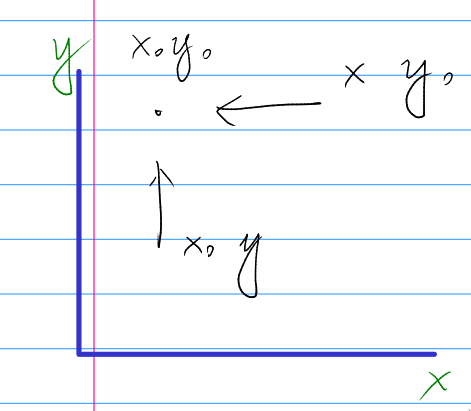
\includegraphics[width=0.8\textwidth]{figures/2021-09-09T203722+0800.png}
\end{marginfigure}
\begin{proof}
	C-R 关系 Cauchy-Riemann equation

	若
	\[
		f'(z) = \lim_{z \to z_0} \frac{ f(z) - f(z_0) }{ z -z_0 } \text{存在} \qc z = x + \im y
	\]
	不论从哪个方向趋于 \( (x_0,y_0) \) 所得都应该是 \( f'(z) \):
	\mn{在欧几里得空间,微小范围,只要从“横平竖直” 两个方向趋近,那么应该是等价的,这里只证明\hl{导数存在 \( \implies \) C-R 关系}}
	\begin{enumerate}
		\item \( (x, y_0) \to (x_0,y_0) \):
		      \begin{align*}
			      f'(z) & = \lim_{z \to z_0} \frac{ f(z) - f(z_0) }{ z -z_0 }                                  \\
			            & =	\lim \frac{  u(x,y_0) + \im  v(x,y_0) - ( u(x_0,y_0) + \im  (v(x_0,y_0)) ) }{x - x_0} \\
			            & = \pdv{u}{x} +  \pdv{\im  v}{x}                                                       \\
			            & = \blue{\pdv{u}{x}} +  \red{\im \pdv{  v}{x}}
		      \end{align*}
		\item \( (x_0, y) \to (x_0,y_0) \):
		      \begin{align*}
			      f'(z) & = \lim_{z \to z_0} \frac{ f(z) - f(z_0) }{ z -z_0 }                                       \\
			            & =	\lim \frac{  u(x_0,y) + \im  v(x_0,y) - ( u(x_0,y_0) + \im  (v(x_0,y_0)) ) }{\im (y - y_0)} \\
			            & = \pdv{u}{\im y} + \pdv{\im v}{\im y}                                                        \\
			            & = \red{- \im  \pdv{u}{y}} + \blue{\pdv{v}{y}}
		      \end{align*}
	\end{enumerate}
	对应项相等有:
	\begin{equation}
		\text{C-R 关系:} \left\{
		\begin{aligned}
			\pdv{u}{x} & = \pdv{v}{y}  \\
			\pdv{u}{y} & = -\pdv{v}{x}
		\end{aligned} \right\}
	\end{equation}
\end{proof}

\begin{equation}
	\oint f(z) \dd{z} = \oint (u+iv)(dx + idy)
\end{equation}
According to Stokes equation:
\begin{equation}
\begin{aligned}
\oint (u+iv)(dx + idy)
&= \oint (udx - vdy) + \im \oint (udy + vdx) \\
&= \int ( \pdv{(-v)}{x} - \pdv{u}{y}  ) \dd{\tau} + \im \int ( \pdv{u}{x} - \pdv{v}{y} ) \dd{\tau} \\
&= 0 + 0 \im
\end{aligned}
\end{equation}

\subsection{平面方程的点法式}%
% \begin{marginfigure}
% 	\begin{center}
% 		\begin{tikzpicture}
% 			\draw[black,thick] (-1,-1) -- (-.06,-.06);
% 			\draw[black,thick] (.06,.06) -- (1,1);
% 			\draw[black,thick] (-1,1) -- (1,-1);
% 			\filldraw[black] (-1,-1) circle (2pt) node[anchor=north] {2};
% 			\filldraw[black] (-1,1) circle (2pt) node[anchor=south] {1};
% 			\filldraw[black] (1,-1) circle (2pt) node[anchor=north] {3};
% 			\filldraw[black] (1,1) circle (2pt) node[anchor=south] {4};
% 		\end{tikzpicture}
% 	\end{center}
% 	\caption{Marginfigure: Tikz}
% \end{marginfigure}
\begin{wrapfigure}{r}{0.30\textwidth}
	\includesvg[width=0.28\textwidth]{figures/平面方程的点法式.svg}
	% \caption{平面方程的点法式}
	% \label{fig:平面方程的点法式}
\end{wrapfigure}
\sn{法向量加一点,确定一个平面}
\begin{marginfigure}
	\begin{flushright}
		\includesvg[width=0.8\textwidth]{figures/平面方程的点法式.svg}
		\caption{平面方程的点法式}
		\label{fig:平面方程的点法式}
	\end{flushright}
\end{marginfigure}
如图~\ref{fig:平面方程的点法式} 所示
\begin{gather*}
	\vb{n} = (A,B,C) \\
	O = (x_0, y_0, z_0)  \\
	P(x,y,z) \\
	\overrightarrow{DP} \perp \vb{n} \\
	(A,B,C) \perp (x-x_0, y-y_0, z-z_0) \\
	A(x-x_0) + B(y-y_0) + C(z-z_0) = 0
\end{gather*}

\begin{equation}
	\label{eq:平面方程的点法式}
	Ax + By + Cz + \underbrace{(- Ax_0 -B y_0 - C z_0 )}_{\text{设为}D} = 0
\end{equation}
\subsection{平面方程的一般式}%
由式~\eqref{eq:平面方程的点法式} 知 平面方程一般式
\begin{equation}
	\label{eq:平面方程一般式}
	Ax + By + Cz + D = 0
\end{equation}
\begin{remark}
	三点确定一个平面。三个点能列出三个方程,故\( A,B,C,D \)中只需要确定三个量就能确定一个平面。\\[2\baselineskip]

	{\itshape 理由:
	\begin{enumerate}
		\item 齐次方程: 只需要算出 \( A,B,C,D \)比例,可以约去
		\item 平面只需要不在同一直线上的三点即可确定
	\end{enumerate}}
\end{remark}
\begin{marginfigure}
	\centering
	\includesvg[width=0.8\textwidth]{figures/condition-of-use.svg}
	\caption{Condition of use}
	\label{fig:condition-of-use}
\end{marginfigure}
Condition of use:
\begin{enumerate}
	\item  The equation can be writen as
	      \( Ax + By + Cz = 0 \),
	      in case the plane \( \Pi \) goes through the origin.
	\item  The equation can be written as \( A x + B y + D =0 \),
	      in case the plane \( \Pi \parallel  Oz \implies C =0 \) (ie. the coefficient of z is 0, C is \( z \) component of the normal vector of \( \Pi \)),
	      as shown as the 1st figure of Fig.~\ref{fig:condition-of-use}
	\item The equation can be written as \( A x + B y =0 \),
	      in case the plane \( \Pi \) goes through the axis \( Oz \)
	      \( \implies
	      \begin{cases}
		      D = 0 \qc \text{goes through the origin} \\
		      C = 0
	      \end{cases}
	      \)
	      , as shown as the 2nd figure of Fig.~\ref{fig:condition-of-use}
\end{enumerate}

\subsection{平面方程的截距式}%
\begin{definition}[平面方程的截距式]
	若平面方程为
	\begin{equation*}
		\frac{x}{a} + \frac{y}{b} + \frac{z}{c} = 1 \quad (a,b,c \neq 0)
	\end{equation*}
	称为截距式。
\end{definition}

该平面经过
\begin{align*}
	(a,0,0) \\
	(0,b,0) \\
	(0,0,c)
\end{align*}
\( a,b,c \)分别为在
\( x \)轴,
\( y \)轴,
\( z \)轴上的截距(不一定为正)

\begin{equation*}
	A x + By +Cz + D =0 \implies
	\frac{x}{- \frac{D}{A}} + \frac{y}{- \frac{D}{B}} + \frac{z}{- \frac{D}{C}} = 1
	\ \ (A,B,C,D \neq 0)
\end{equation*}

\subsection{平面方程三点式}%
若平面 \( \Pi \)经过不在同一直线上的三点,
\(
M_1(x_1,y_1,z_1),
M_2(x_2,y_2,z_2),
M_3(x_3,y_3,z_3),
\)
或
\(
\mqty[
	x_1&y_1&z_1 \\
	x_2&y_2&z_2 \\
	x_3&y_3&z_3
]
\)
线性无关,求平面 \( \Pi \)的方程。

解法一:
\begin{equation}
	\mqty[
		x_1 & y_1 & z_1 & -1 \\
		x_2 & y_2 & z_2 & -1 \\
		x_3 & y_3 & z_3 & -1
	]
	\mqty[
		A \\ B \\ C \\ D
	]
	=0
\end{equation}

% 	\centering
% 	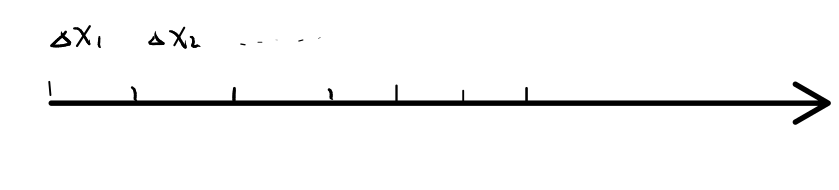
\includegraphics[width=0.8\linewidth]{figures/2021-09-05T122541+0800.png}
% 	\caption{等距分布}%
% \end{figure}
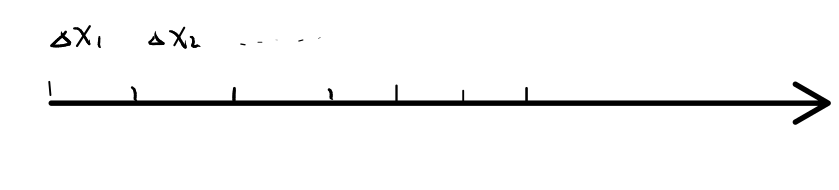
\includegraphics[width=0.8\linewidth]{figures/2021-09-05T122541+0800.png}
\begin{itemize}
	\item 用 \( i \)还是 \( j \)其实无所谓,\( i \) 从 \( 0 \) 取到 \( n \),\( n \) 的大小也无所谓
	\item \( \Delta x_i \)的大小无所谓,只需要 最大的那段\( \max(\{ \Delta x_i, i \in [1, n] \}) \to 0 \)
	\item 所需要表示的只是对应的\emph{加权}的和的极限
	      \begin{enumerate}
		      \item 对应相乘 \(\Delta \psi_i = f_i \vdot \Delta x_i \)
		      \item 求和 \( \sum_i \Delta \psi_i \)
		      \item 取极限 \( \lim_{\max(\{ \Delta x_i \}) \to 0} \sum_i \Delta \psi_i \)
	      \end{enumerate}
\end{itemize}
所以简化书写把\( i \)去掉
\begin{enumerate}
	\item 每一项写成 \( \dd \psi = f \dd x \)
	\item 求和写成 \( \int \dd \psi \)
\end{enumerate}
